\documentclass[12pt, a4paper]{article}
\usepackage[utf8]{inputenc}
\usepackage{amsmath}
\usepackage{amsthm}
\usepackage{graphicx}
\usepackage{parskip}
\usepackage{titling} 
\usepackage{hyperref}
\usepackage{fancyhdr}
\usepackage{lastpage}
\graphicspath{ {./images/} }
\title{
  Lab Session 1 - Answers \\
  AMMM
}
\author{Juan Pablo Royo Sales}
\date\today

\pagestyle{fancy}
\fancyhf{}
\fancyhead[C]{}
\fancyhead[R]{Juan Pablo Royo Sales - UPC MIRI}
\fancyhead[L]{AMMM - Lab Session 1}
\fancyfoot[L,C]{}
\fancyfoot[R]{Page \thepage{} of \pageref{LastPage}}
\renewcommand{\headrulewidth}{0.4pt}
\renewcommand{\footrulewidth}{0.4pt}

\begin{document}

\begin{titlingpage}
  \maketitle
\end{titlingpage}

\section{Answers}
\subsection{Answer 1}\label{answer_1}

Formula 1 state that $\forall c \in C$ we are doing the following:


\begin{itemize}
  \item $\forall t \in T$ we are adding up the fraction of resource requested by
    $t$ on $c$ by the amount of requested resources by task $t$.
  \item That summation we are dividing by the processing capacity of that $c$
\end{itemize}

Therefore we cannot assign to each processor more that its own capacity. If we
are taking the maximum we cannot take more that maximum load of the whole set of processors.


\subsection{Answer 2}

We have run 3 different data set apart from the default.

\subsubsection{Default Data Set}

Here we can see the data used

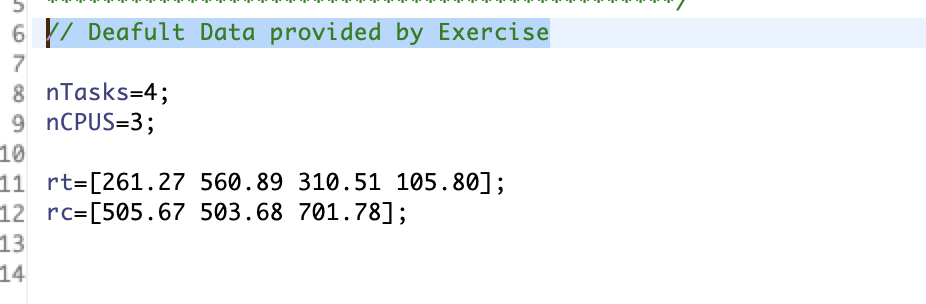
\includegraphics{deafult_data}

Here we can see the result of the model based on that data

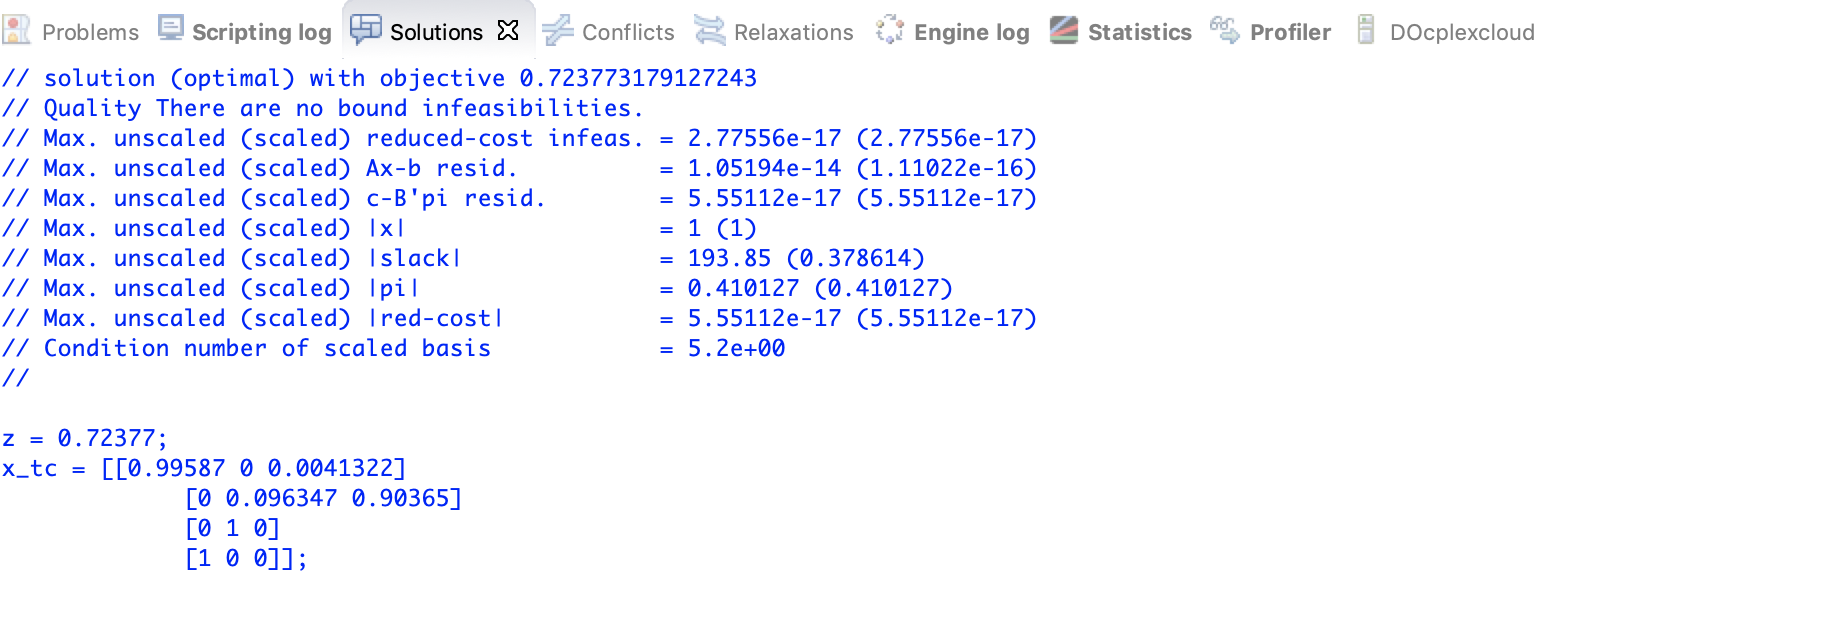
\includegraphics[width=\textwidth]{output_default_data}

\subsubsection{Data Set 2}

In this data set we have assigned one CPU with high capacity, other with low and
other with mid capacity.

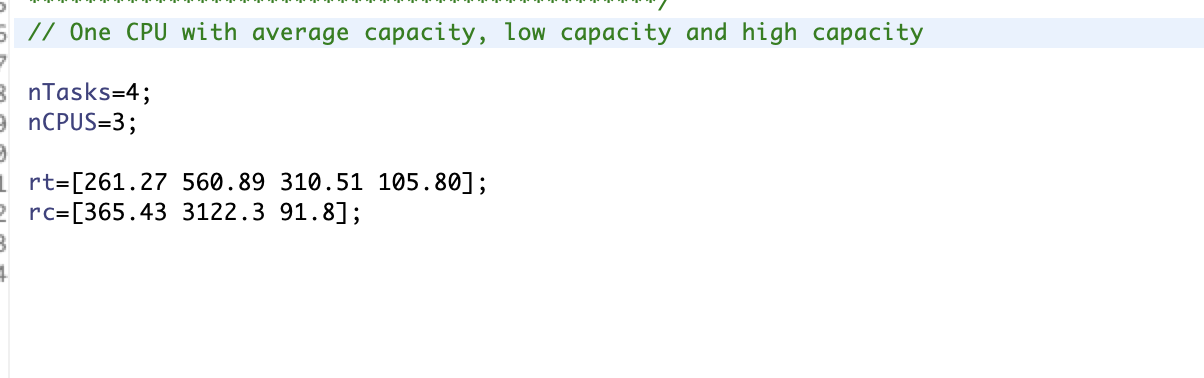
\includegraphics{data_2}

This is the output result

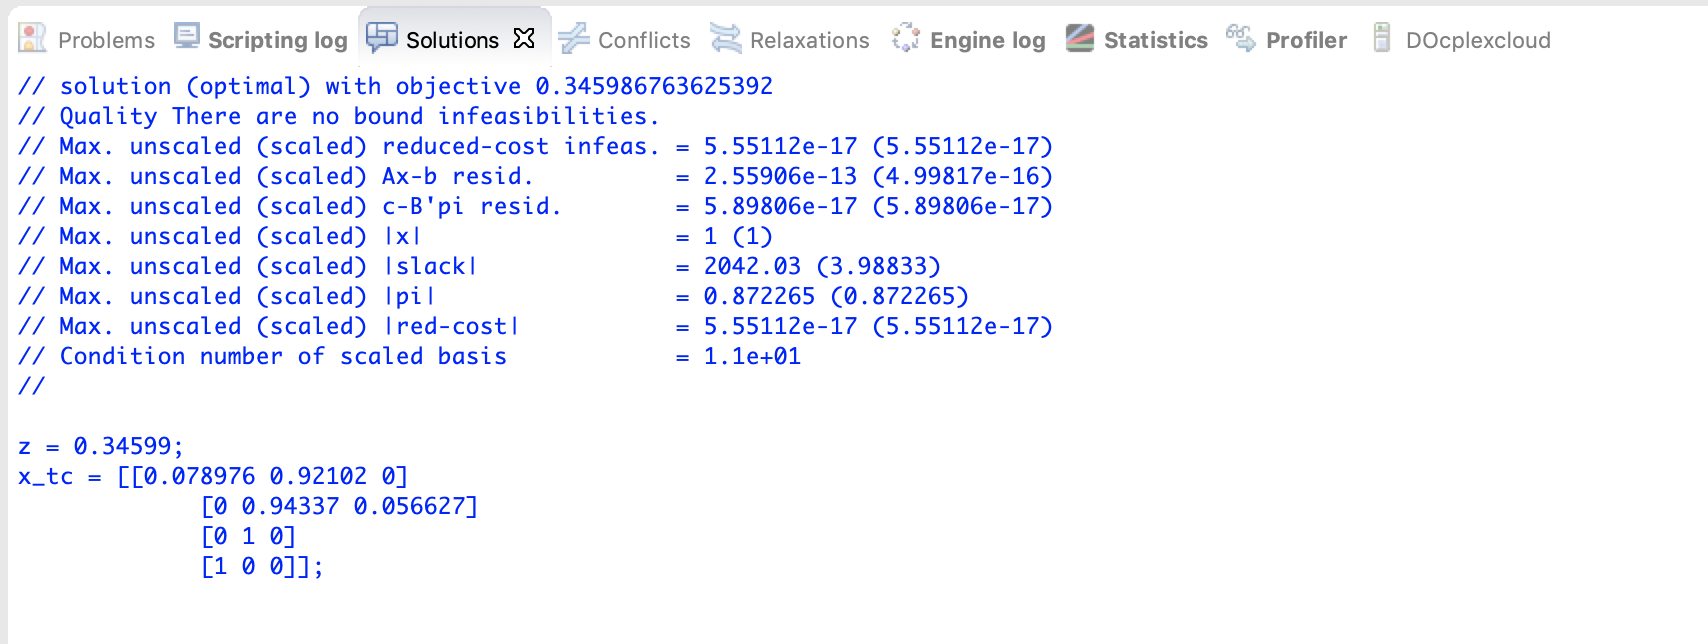
\includegraphics[width=\textwidth]{output_data_2}

As we can appreciate here, $z$ has decreased from $72\% $ to $35\%$. This is
because we have set a CPU with high capacity we also have another CPU with
average capacity. In this sense since $z$ is the maximum of the capacities as we
have shown in \ref{answer_1} we have more CPU capacity available.

\subsubsection{Data Set 3}

In this data set we have set all the CPU with high capacity like the following:

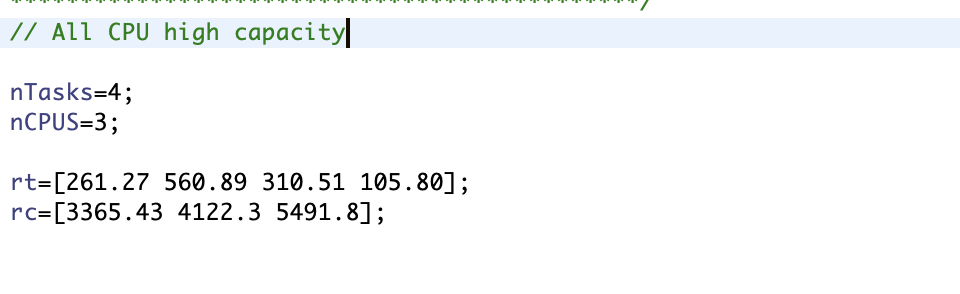
\includegraphics{data_3}

This is the output result

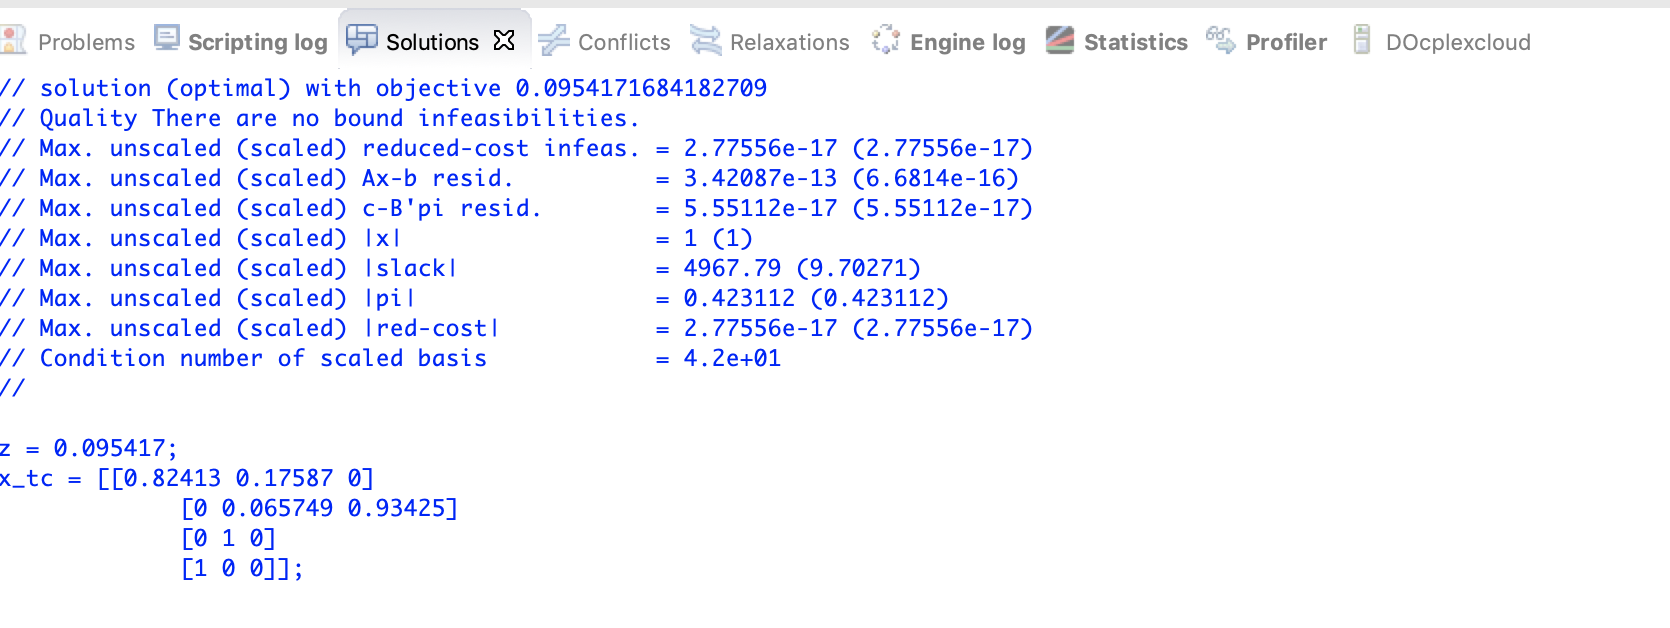
\includegraphics[width=\textwidth]{output_data_3}

As we can see here since we have a lot of CPU capacity available $z$ has
decreased to $9\%$

\subsection{Answer 3}

If we decrease one of the CPU capacity, this capacity should be reduced until
$229.13$ before reaching unfeasibility.

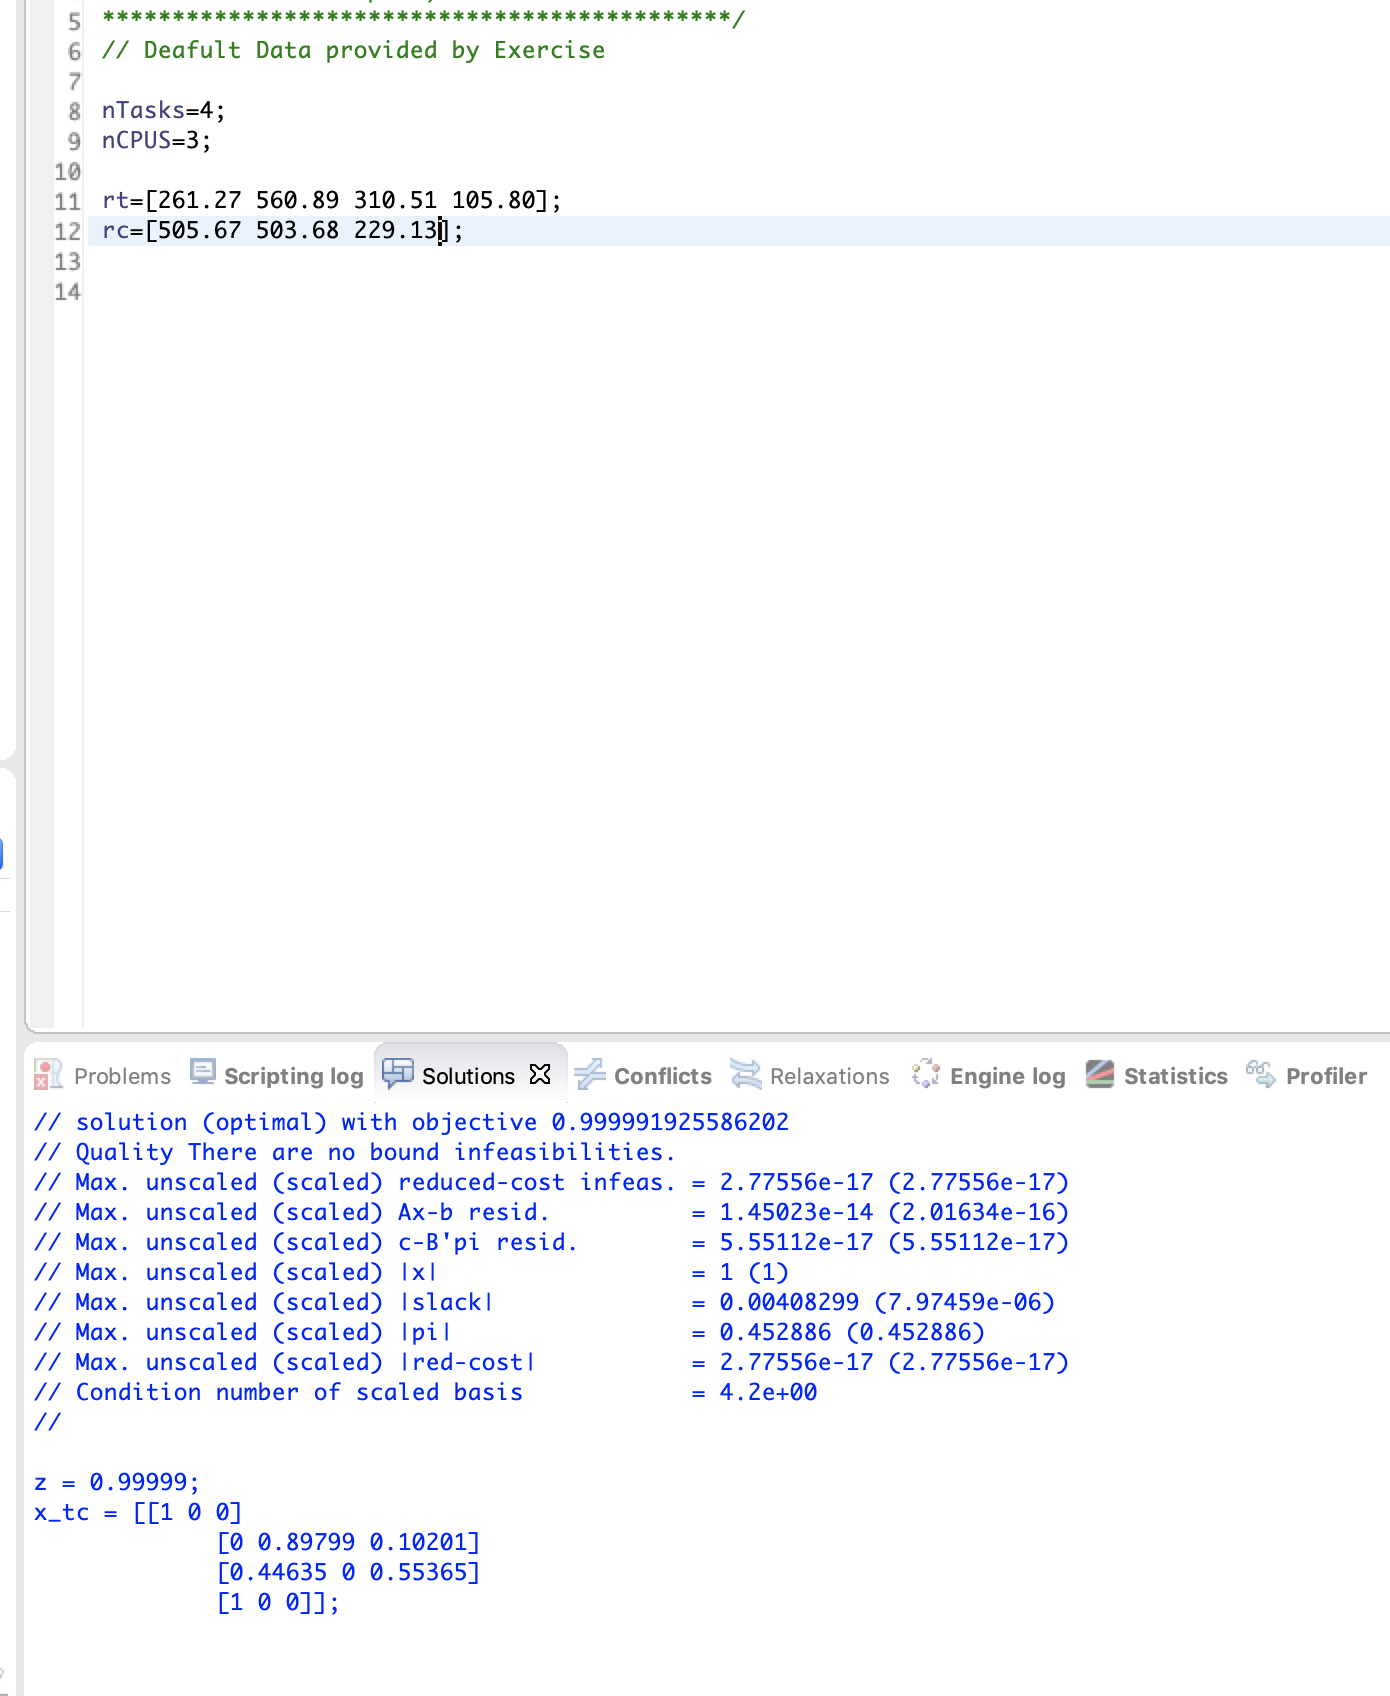
\includegraphics[width=\textwidth]{unfeasible}

If we decrease a little more we reach the unfeasibility

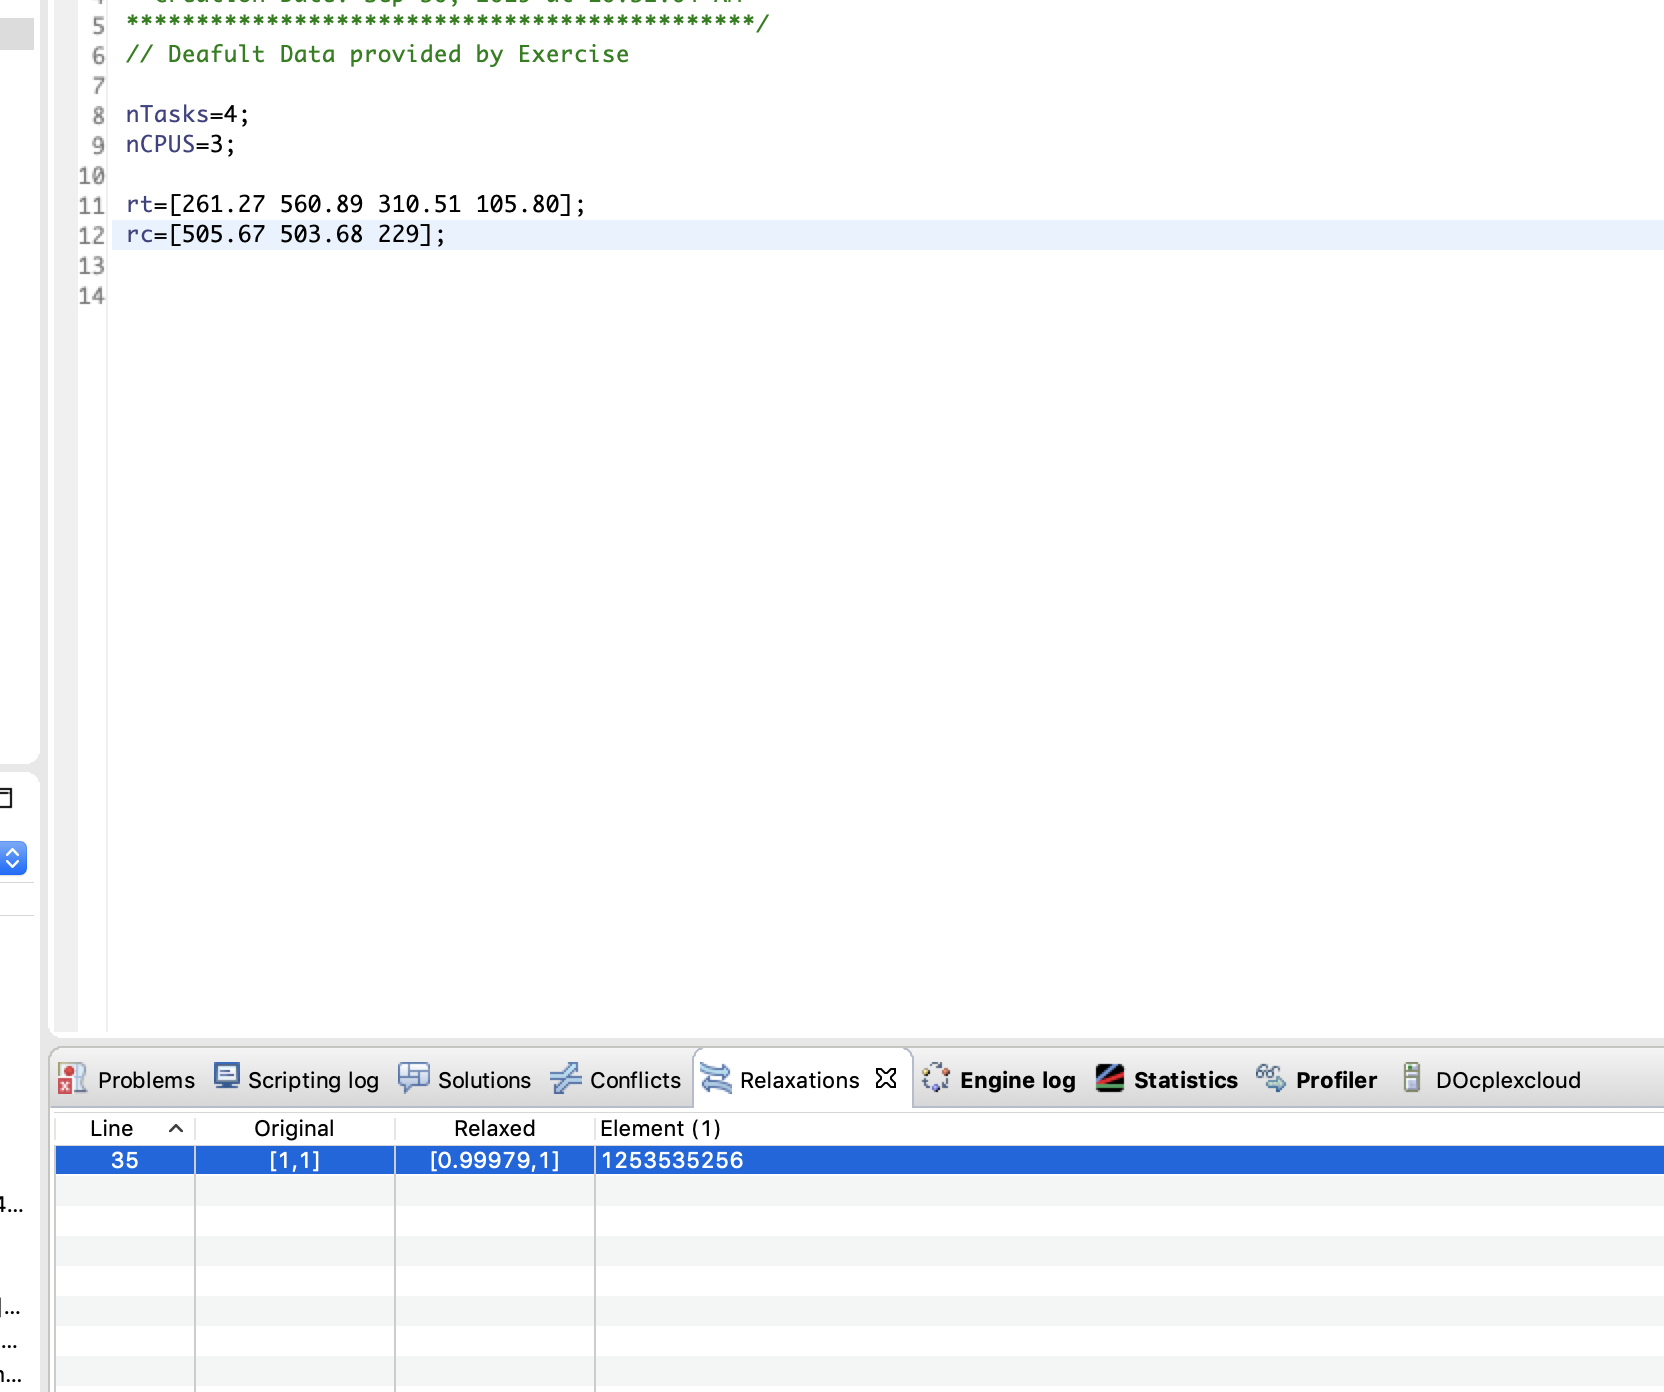
\includegraphics[width=\textwidth]{increase_unfesible}

This can be deduce by the first constraint which summation should be equal to 1.

In this sense if we do the calculations but with last CPU as unknown we can
easily get 229.13 value.

Lets see:

\begin{subequations}
  \begin{align}
  rt = 261.27 + 560.89 + 310.51 + 105.80 = 1238.47 \\
  rc = 505.67 + 503.68 + c_3 = 1238.47 \\
  c_3 = 219.13
  \end{align}
\end{subequations}

Therefore, to minimize $z$ to be 1 which is still feasible $c_3$ could not be
less than $219.13$

\end{document}